% !TEX TS-program = pdflatex
% !TEX encoding = UTF-8 Unicode

% This is a simple template for a LaTeX document using the "article" class.
% See "book", "report", "letter" for other types of document.

\documentclass[11pt]{article} % use larger type; default would be 10pt

%\usepackage[utf8]{inputenc} % set input encoding (not needed with XeLaTeX)


%%% Examples of Article customizations
% These packages are optional, depending whether you want the features they provide.
% See the LaTeX Companion or other references for full information.

%%% PAGE DIMENSIONS
\usepackage{geometry} % to change the page dimensions
\geometry{a4paper} % or letterpaper (US) ocher a5paper or....
\geometry{margin=1in} % for example, change the margins to 2 inches all round
% \geometry{landscape} % set up the page for landscape
%   read geometry.pdf for detailed page layout information

\usepackage{graphicx} 
% \usepackage[parfill]{parskip} % Activate to begin paragraphs with an empty line rather than an indent

%%% PACKAGES
%\usepackage{booktabs} % for much better looking tables
\usepackage{array} % for better arrays (eg matrices) in maths
%\usepackage{paralist} % very flexible & customisable lists (eg. enumerate/itemize, etc.)
\usepackage{verbatim} % adds environment for commenting out blocks of text & for better verbatim
%\usepackage{subfig} % make it possible to include more than one captioned figure/table in a single float
% These packages are all incorporated in the memoir class to one degree or another...

%%% HEADERS & FOOTERS
\usepackage{fancyhdr} % This should be set AFTER setting up the page geometry
\pagestyle{fancy} % options: empty , plain , fancy
\renewcommand{\headrulewidth}{0pt} % customise the layout...
\lhead{}\chead{}\rhead{}
\lfoot{}\cfoot{\thepage}\rfoot{}

%%% SECTION TITLE APPEARANCE
%\usepackage{sectsty}
%\allsectionsfont{\sffamily\mdseries\upshape} % (See the fntguide.pdf for font help)
% (This matches ConTeXt defaults)

%%% ToC (table of contents) APPEARANCE
%\usepackage[nottoc,notlof,notlot]{tocbibind} % Put the bibliography in the ToC
%\usepackage[titles,subfigure]{tocloft} % Alter the style of the Table of Contents
%\renewcommand{\cftsecfont}{\rmfamily\mdseries\upshape}
%\renewcommand{\cftsecpagefont}{\rmfamily\mdseries\upshape} % No bold!

%\usepackage[T1]{fontenc}
\usepackage[latin9]{inputenc}
%\usepackage[active]{srcltx}
\usepackage{setspace}
\doublespacing
\usepackage[english]{babel}

\begin{document}

\title{Connectivity Analysis of Metagenomic Data}
\author{ACH, JP, RCK, RM, ST, JJ, JMT, CTB}
\maketitle

\section{Introduction}
Given the rapid decrease in the costs of sequencing, we can now achieve the sequencing depth necessary to study even the most complex environments \cite{Hess:2011p686,Qin:2010p189}.  High throughput, deep metagenomic sequencing efforts in permafrost soil, human gut, cow rumen, and surface water have provided insights into the genetic and biochemical diversity of environmental microbial populations \cite{Hess:2011p686,Iverson:2012p1281,Qin:2010p189} and the extent to which they are involved in responding to environmental changes \cite{Mackelprang:2011p1087}. These metagenomic studies have all leveraged \emph{de novo} metagenomic assembly of short reads to assign sequences to microbial taxa and function.  \emph{De novo} assembly is an advantageous approach to sequence analysis as it reduces the dataset size by collapsing numerous short reads into fewer contigs and provides longer sequences containing multiple genes and operons \cite{Miller:2010p226,Pop:2009p798} making annotation-based approaches more practical.  Furthermore, it does not rely on the availability of reference genomes to enable identification of novel genetic features and draft genomes \cite{Hess:2011p686,Iverson:2012p1281}.

Although \emph{de novo} metagenomic assembly is a promising approach for deep sequencing of metagenomes, it is complicated by the variable coverage of sequencing reads from mixed populations in the environment and their associated sequencing errors and biases \cite{Mende:2012p1262,Pignatelli:2011p742}. Several metagenomic-specific assemblers have been developed to deal with variable coverage communities, including Meta-IDBA \cite{Peng:2011p898}, MetaVelvet, and SOAPdenovo.  These assemblers rely on local models of sequencing coverage to help build assemblies and thus are sensitive to the effects of sequencing errors and biases on coverage estimations of the underlying dataset. The effects of sequencing errors on \emph{de novo} assembly has been demonstrated in simulated metagenomes \cite{Mavromatis:2006p894,Mende:2012p1262,Pignatelli:2011p742}, but these datasets do not incorporate models that are representative of real metagenomic data.  Specifically, these models exclude the presence of of known non-biological sequencing biases \cite{GomezAlvarez:2009p1334,Niu:2010p1333} which would hinder coverage-based assembly approaches.  

In this study, we examine real metagenomic datasets for the presence of these artificial sequencing biases, extending previous work to large and complex datasets produced from the Illumina platform. Since these sequencing biases would erroneously connect numerous reads together, they can be characterized by their connectivity within an assembly graph.  Here, we take advantage of a de Bruijn assembly graph representation to identify and evaluate highly connective sequences within various metagenomic datasets.  We demonstrate that there exist highly connective sequences which originate, at least partially, from sequencing artifacts, and examine the effects of removing these sequences to minimize their incorporation into resulting assemblies.

\section{Results}

\subsection{Connectivity analysis of metagenome datasets}

\subsubsection{Presence of a single, highly-connected lump in all datasets}
We selected datasets from three diverse, medium to high diversity metagenomes from the human gut \cite{Qin:2010p189}, cow rumen \cite{Hess:2011p686}, and agricultural soil, representing metagenomes sequenced to various depths (Table 1).  To evaluate the effects of sequencing coverage, we also included lower-coverage subsets of the soil metagenome (520 million reads),  a subset with 1.4\% coverage (50 million reads) and another with 4.7\% coverage (100 million reads).  We also included a previously published error-free simulated, metagenome based on a mixture of 112 reference genomes \cite{Pignatelli:2011p742}.

Initially, we evaluated the amount of connectivity between all sequences in each metagenome, similar to the initial step of all current short read assemblers to identify the connectivity of short sequences of length 'k', or k-mers \cite{Peng:2011p898,Simpson:2009p233,Zerbino:2008p665}.  For complex metagenomes, extremely large diversity and numerous sequencing errors require large amounts of memory to store the resulting assembly graph \cite{Hess:2011p686,Mackelprang:2011p1087,Qin:2010p189}.  To overcome this limitation, we constructed a probabilistic representation of the assembly graph using a bloom filter de Bruijn graph representation within fixed memory as previously described (Pell et al, how to cite this?).  

Using this assembly graph representation, we separated reads contributing to disconnected portions of the metagenome assembly graph (e.g., representatives from separate populations in the source environment).  For each metagenome, regardless of origin, we found a single dominant, highly-connected set of sequencing reads which we henceforth refer to as the  "lump"  of the dataset (Table 1).  This lump contained the largest subset of connected sequencing reads and varied in size among the datasets, ranging from 5\% of total reads in the simulated metagenome to 75\% of total reads in the human gut metagenome (Table 1).  For the soil datasets, as sequencing coverage increased from 1.4\% to 4.7\% to 5.6\%, the lump size increased more dramatically from 7\% to to 15\% to 35\% of the total reads, indicating increasingly larger connectivity between sequences with more sequencing.

\subsubsection{Characterizing the dominant lump within the assembly graph}

Given the large number of reads connected within metagenomic lumps (up to 262 million reads in the human gut dataset), we quantified the degree of connectivity of sequences within the lump by estimating the average local graph density from nodes in the assembly graph (See Methods).  We observed that sequences in the identified metagenomic lumps had very high local graph densities, between 22 to 50\% of the total nodes in metagenomic lump assembly graphs had average graph densities greater than 20 (Table 1).  In comparison, 17\% of the total nodes in the simulated lump had an average local graph density greater than 20, and a mixture of the 112 source genomes for the simulated dataset had fewer than 2\% of its nodes with an average graph density greater than 20.  The unusual high graph densities observed within the metagenomic lumps relative to both the simulated lump and mixture of genomes suggested anomalous connectivity within associated reads.  

We next assessed the extent to which graph density varied by position along the sequencing reads.  The degree of position-specific bias of graph densities was estimated by calculating the average local graph density within ten steps of every k-mer by position in each read.  In all environmental metagenomic reads, we observed biases in graph density at the 3'-end region of reads (Figure 1).  In soil metagenomes, we observed the most dramatic biases with estimated local graph density increasing at the 3'-end of the reads.  Notably, this bias was not present in the simulated dataset.  Next, we identified specific sequences within dense regions of the assembly graph which consistently contributed to high connectivity in an exhaustive graph traversal of the reads within each lump.  We observed that this subset of sequences were also found to exhibit position-specific biases within sequencing reads (Figure 1, solid lines).  Similar to local density trends, position-specific biases of these sequences also varied between metagenomes.  As sequencing coverage increased among metagenomes, the amount of 3'-end bias appeared to decrease (e.g., the soils) or inverse (e.g., rumen and human gut), and in the case of the simulated dataset, no such biases were observed.

\subsection{Effects of removal of highly connective sequences on assembly}

In all datasets, we found that our approaches for removal of highly connective k-mers was effective at breaking apart metagenomic lumps (Table 1), and the resulting size of the largest partition of connected reads in each metagenome was reduced to less than 7\% of the total reads in the lump.  The partitioned sets of sequences could be assembled very efficiently in parallel, greatly reducing the memory and time required for assembly to less than 2 Gb memory  and less than 1 hour  for all metagenomes.  For the largest soil dataset, assembly was reduced from X to X.   

To explore the extent to which the identified highly-connective sequences impacted assembly, we first evaluated the effects of the removing these sequences from reads in the simulated lump and its resulting assemblies.  The assemblies of the reads in the original simulated lump (the unfiltered assembly) and the reads remaining after removing highly connective sequences (the filtered assembly) were compared for three assemblers (Velvet, Meta-IDBA, and SOAPdenovo).  Based on total assembly length of contigs greater than 300 bp, filtered assemblies of the simulated metagenome resulted in a loss of between 4 - 16\% of total assembly length (Table 2).  Overall, filtered assemblies contained fewer total contigs than unfiltered assemblies, and the maximum contig size increased in the case of Velvet assembly but decreased in the case of the Meta-IDBA and SOAPdenovo assemblies.  Direct comparisons of two assemblies showed that the filtered assembly comprises about on average 88\% of the unfiltered, and the unfiltered contains nearly all (96\%) of the filtered assembled sequences.  Despite the removal of over 3\% of the total unique 32-mers in the simulated metagenome, these resulting filtered assemblies resulted in only a loss of 0.1 - 0.6\% of original reference genes. 

We next evaluated the effects of using similar approaches in metagenomic datasets.  Similar to the simulated assemblies, the removal of highly connective sequences for all metagenomes and assemblers resulted in a loss of total assembly length and number of contigs.  In general, filtered assemblies were for the large part contained within unfiltered assemblies and comprised 67-88\% of unfiltered assembly.   The observed changes in metagenomic assemblies were difficult to evaluate as the source genomes to these datasets are unknown, and a loss in assembly length may actually be beneficial due to the elimination of artifactual contigs.  To aid in this evaluation, we used the previously published set of rumen draft genomes which were constructed from \emph{de novo} assembly efforts of the rumen metagenome \cite{Hess:2011p686}.  Overall, we found that removal of highly connective sequences from the rumen dataset resulted in 1-3\% loss of sequences which matched to the draft reference genomes.  To further study the effects of highly connective sequences, we examined their incorporation into unfiltered assemblies.  Each assembled contig was divided into equal length bins (the size of bins was dependent on the total length of the contig) and examined for the presence of the previously identified highly connective sequences.  Overall, we found that assembled contigs, regardless of assembler, placed a larger fraction of these sequences on the ends of its contigs relative to other binned positions.

\subsubsection{Characterizing highly connective sequences}

For the simulated metagenome, we could identify the original source of highly connective k-mers using the available reference genomes.  Many of these sequences originated from well-conserved housekeeping genes involved in protein synthesis, cell transport, and signaling.  The top reference genes identified with perfect matches to highly connective k-mers which were present in the dataset a minimum of 50 times are shown in Table 3.  To determine possible biological sources of highly connective sequences within real metagenomes, we compared the sequences shared between the soil, rumen, and human gut metagenomes.  In total, 7,586 highly-connecting sequences (32-mers) were shared between the three soil, rumen, and human gut metagenomes.  We identified the closest reference protein from the NCBI-nr database requiring complete sequence identity.  Only 1,018 sequences (13\%) matched existing reference proteins, and many of the annotated sequences matched multiple conserved protein sequences from multiple genomes.  The top five proteins conserved in greater than 3 genomes are shown in Table 4, and largely encode for genes involved in protein biosynthesis, DNA metabolism, and biochemical cofactors (Table 4).

A potential cause of artificial high connectivity within metagenomes is the presence of high abundance sequences.  Thus, we identified the subset of highly connective k-mers which were also present with an abundance of greater than 50 within each metagenome (Figure 1, dotted lines).   These high abundance k-mers comprised a very small proportion of the identified highly connective sequences, less than 1\% in the soils, 1.5\% in the rumen, and 6.4\% in the human gut metagenomes, but the position-specific biases of these sequences were very similar to the biases of the larger set of highly connective k-mers.

To identify consistent patterns within sequences causing position-specific biases, we examined the abundance of distribution unique 5-, 6-, 7-, 8-mers contained within the high abundance subset of each dataset's highly connective k-mers. 

\section{Discussion}

\subsection{Highly connected assembly subgraph contains sequencing artifacts.}

Through assessing the connectivity of reads in several metagenomes, we identified a disproportionately large subset of reads which were connected together within an assembly graph, hereafter referred to as the "lump" in each metagenome.  The simulated metagenome's lump comprised 5\% of its total reads (Table 1).  As this dataset contains no errors, this observed connectivity represents conserved sequences within a single genome or between multiple genomes (Table 2).  In contrast, the highly connective lump within real metagenomic lumps comprised a significantly larger proportion of reads, ranging from 7\% to 75\% of the total reads (Table 1), suggesting that anomalous, non-biological connectivity may be present within these lumps.  Interestingly, in the soil metagenomes, we observed that the amount of connectivity nearly doubled with less than a 5\% increase of sequencing coverage.  Given the very high diversity and very low coverage of these soils, the magnitude of this increase seemed unlikely from biological sources, further supporting the presence of sequencing biases within these datasets. 

If sequencing biases were present within these metagenomes, we would expect to observe that the metagenomic lumps would consist not only of artificial sequences but also sequences from reads which would be "preferentially attached" \cite{Barabasi:1999p1083}.  Consider that there is an original set of highly connecting "X" sequences in a lump.  These sequences would recruit a number of connective "Y" reads into the lump.  These recruited "Y" reads would then recruit more "Z" reads into the lump which would not necessarily connect to the original "X" reads.  In error-free datasets, we would observe this preferential attachment phenomenon as a linear increase of lump size with increasing sequencing coverage.  In the case of the presence of highly-connective sequencing biases, however, we'd observe that preferential attachment would cause dramatic increases in the number of recruited "Y" and "Z" reads, such is the observed case in the soil datasets.   

To more rigorously demonstrate the presence of artifacts within our datasets, we considered that the sequencing of metagenomes is a random process and thus any position-specific bias within sequencing reads is unexpected and non-biological.   For the metagenomes studied here, we used two approaches to examine characteristics of connectivity correlated to specific positions within sequencing reads.  First, we measured the local graph density (as defined in Methods) at specific positions within sequencing reads.  Next, we identified the specific k-mers which were consistently present in highly dense regions of the assembly graph and evaluated their location within sequencing reads.  When these approaches were applied to the simulated dataset, we observed no position-specific trends when assessing either local graph density (Figure 1) or highly connective k-mers (Figure 2), as is consistent with the lack of sequencing errors and biases in this dataset.  In all real metagenomes, however, we identified position-specific trends in measurements of both local graph density and the location of highly connective sequences, clearly indicating the presence of artificial sequences.  Although present in all metagenomes, the direction of the bias varied between soil, rumen, and human gut datasets, particularly for the position-specific presence of highly connective sequences.  It is possible that in higher coverage datasets, such as the rumen and human gut, there is a larger presence of indirectly preferentially attached reads which are connected to high coverage sequences of biological origins.  Thus, as the total number of sequences associated in a lump is used to calculate the fraction of highly connective k-mers (Figure 1, y-axis), preferential attachment would result in increasing the number of total reads and effectively decrease the total fraction of highly connective reads.  This trend is observed in the decreasing fractions of highly connective sequences as sequencing coverage increased in the small, medium, to large soil metagenomes and in the soil, rumen, to human gut metagenomes.

\subsection{Removal of highly connective sequences results in similar assemblies in the simulated dataset lump.}

As is apparent from conserved biological sources of high connectivity within the simulated metagenome, not all the observed connectivity within real metagenomes is artificial, and our approaches are limited in that they cannot differentiate between sequencing artifacts and sources of real biological connectivity.  Regardless of the origin of highly connective sequences, we suspected that these sequences would challenge assemblers which rely on resolving the complexity of an assembly graph.  Consequently, we evaluated the incorporation of these sequences in assembled contigs and found that they were disproportionately placed at the ends of contigs (Figure 3), suggesting that assembly could not extend beyond these sequences.  Considering that these sequences displayed position-specific bias and challenged assemblers, we removed them from metagenomic lumps.  Unsurprisingly, the removal of highly connective sequences resulted in the dissolution of high connectivity within the lump and several smaller sets of connected reads.  

We compared the combined assembly of these partitioned sets of reads to the original lump dataset with several assemblers.  A key advantage to removing highly connective sequences was the ability to assemble smaller subsets of reads in parallel, resulting in significantly reduced assembly requirements (time and memory) (Table 2).  For the assemblies of the large soil and human gut metagenomes, multiple k-mer length assemblies and merging of resulting assembled contigs could not be completed in available memory.  Removal of highly connective sequence not only enabled their assembly but also allowed for using multiple and/or separate assembly parameters and various assemblers for different partitions.  The ability to efficiently evaluate multiple assemblies (with a variety of parameters) will be increasing important as metagenome sizes quickly grow larger. 

The advantages of removing highly connective sequences must be balanced against consequences to resulting assemblies.  Here, we have compared several metagenome assemblies before and after the removal of these sequences.  We have previously demonstrated that high abundance, highly connective artificial sequences are present in each metagenome and incorporated into assemblies, resulting in questionable contigs.  Consequently, we know we are comparing filtered assemblies against original assemblies of unknown quality, with the exception of the simulated metagenome where reference genomes can be used for evaluation.  Comparing the simulated dataset's assemblies, the removal of highly connective sequences resulted in very few losses of annotated reference genes and a similar assembly compared to the unfiltered data (~85\% similarity), supporting the removal of these highly connective sequences.  For the rumen metagenome, we could do partial evaluation of the assemblies using draft reference genomes previously constructed from the assembly of high abundance k-mers from the original published dataset.  Similar to the simulated data, we observed only a small loss of reference genomes assembled (Table 2).  In general, for all metagenomes, we observed ~25\% loss in assembly after removing highly connective sequences, much more than observed in assemblies of reference genes and genomes in the simulated and rumen datasets.  This evidence suggests that it is likely that some portion of the loss of assembled contigs is a result of removing misassembled sequences resulting from the presence of sequencing artifacts.

\subsection{Possible origins of highly connective sequences.}

Having targeted specific sequences to remove for assembly, we attempted to identify any biological characteristics of these sequences.  In identifying the highly connective sequences in the simulated dataset and those shared by all metagenomes, we identified that a small portion of these sequences (13\% in simulated and < 7\% in metagenomes) matched reference genes and were mostly associated with housekeeping functions (Tables 3 and 4).   We speculated that the remaining highly connective sequences could originate from high abundance reads, originating from biological sources of high connectivity or sequencing biases.  To study the effects of sequencing biases, we selected the subset of sequences which were extremely abundant (greater than 50x) in the datasets and found that these sequences displayed similar trends for position-specific biases compared to their respective sets of highly connective sequences (Figure 3), indicating that they are comprised of sequencing biases.  To identify characteristics of possible sequencing biases, we next evaluated signatures in high abundance, highly connective sequences by examining the distribution of short length k-mers.  For all metagenomes, we found little bias towards specific k-mers, suggesting that these sequences are largely random rather than characterized by specific motifs. 

\section{Conclusion}

As datasets from NGS technologies continue to increase in size, our ability to analyze this sequencing data must reevaluated.  Here, we demonstrate the presence of sequencing artifacts within several metagenomic datasets that are a cause of non-biological connectivity within assembly graphs.  We show that the abundant, highly connective sequences are sources of sequencing artifacts in metagenomes.  These sequences add erroneous diversity and high coverage into metagenomes, significantly increasing memory requirements for de novo assembly.  Our previous efforts to resolve components of complex metagenome assembly graphs have been bottlenecked by the presence of highly-connective sequences that are have both biological and artificial origins.  Here, we have developed approaches to identify these sequences and demonstrate that their removal results in comparable assemblies.  Importantly, the removal of such sequences results not only in eliminating artificial sequences but also allows for the partitioning of disconnected subgraphs, significantly reducing assembly requirements.  Our analysis provides an understanding of the nature of these sequences and how their removal is an important first step for scalable \emph{de novo} assembly.  As datasets from NGS technologies continue to increase in size, this study highlights the importance of re-evaluating the nature of new sequencing data for both accurate and efficient downstream analysis approaches. 

\section{Methods}

\subsection{Metagenomic datasets}
All datasets, with the exception of the agricultural soil metagenome, originate from previously published datasets. Rumen-associated sequences (Illumina) were randomly selected from the rumen metagenome available at ftp://ftp.jgi-psf.org/pub/rnd2/Cow\_Rumen \cite{Hess:2011p686}. Human-gut associated sequences (Illumina) of samples MH0001 through MH0010 were obtained from ftp://public.genomics.org.cn/BGI/gutmeta/Raw\_Reads \cite{Qin:2010p189}.  The simulated high complexity, high coverage dataset was previously published (Pignatelli, 2011).  All reads used in this study, with the exception of those in simulated metagenome, were quality-trimmed for Illumina's read segment quality control indicator, where a quality score of 2 indicates that all subsequent regions of the sequence should not be used. After quality-trimming, only reads with lengths greater than 30 bp were retained. All quality trimmed datasets, including the previously unpublished agricultural soil metagenome, are available on a public Amazon EC2 snapshot, XXX.   The number of reads after quality-trimming is shown in Table 1 for each metagenome.  The sequencing coverage of each metagenome was estimated as the fraction of reads which could be aligned to assembled contigs with lengths greater than 500 bp.  For the coverage estimates, an assembly of each metagenome was performed using Velvet (v1.1.05) with the following parameters:  K=33, exp cov=auto, cov cutoff=0, no scaffolding.  Reads were aligned to assembled contigs with Bowtie (v0.12.7), allowing for a maximum of two mismatches.  

\subsection{Lightweight, compressible de Bruijn graph representation}
We used a lightweight probabilistic de Bruijn graph representation to explore k-mer connectivity of the assembly graph (cite PNAS paper, software available at https://github.com/ctb/khmer). The de Bruijn graph stores k-mer nodes in Bloom filters and keeps edges between nodes implicitly, i.e. if two k-mer nodes exist with a k-1 overlap, then there is an edge between them. Bloom filters are a probabilistic set storage data structure with false positives but no false negatives, thus the size of the bloom filters were selected to be appropriate for each dataset and the memory available.  For analyzing the graph connectivity of the studied datasets, we used 4 x 48e9 bit bloom filters.  As metagenomic sequencing contains a mixture of multiple organisms, we could exploit the biological structure of the sequencing by partitioning the assembly graph into disconnected subgraphs that represent the original DNA sequence components. The set of the largest number of reads which were connected in the assembly graph is referred to above as a single, highly-connected lump.  Examples of scripts used for this analysis are available on the Amazon EC2 public snapshot:  method-examples/0.partitioning-into-lump.

\subsection{Local graph density and identifying highly-connected k-mers}
We implemented a systematic traversal algorithm to identify highly connected components of the assembly graph.  Waypoints were labeled to cover the graph such that they are a minimum distance of L apart. Originating from a waypoint, all k-mers (throughout the study k=32) were systematically and exhaustively traversed within a region that is the distance N.  The local graph density was calculated as the number of X k-mers reachable within a distance of N nodes (k-mers) divided by the distance N.  In this study, N was equal to 10 nodes within the assembly graph.  For the largest metagenomes, the metahit and large soil datasets, local graph density was calculated on a representative subset of reads due to computational limitations.  To identify specific highly-connective sequences within the lump assembly graphs, graph traversal to a distance of 40 nodes was attempted from marked waypoints.  If more than 200 k-mers were found within this traversal were identified, all k-mers within this traversal were identified as candidates for highly connective sequences.  If the same k-mers were consistently identified in other graph traversals, up to five times, the k-mer was flagged as a highly connective sequence.  Aligning theses k-mers to original sequencing reads, we identified the position-specific location of these k-mers.  To evaluate the effects of these k-mers on assembly, sequencing reads were trimmed at the location where a highly connective k-mer could be aligned and the resulting assemblies are referred to as "filtered" assemblies.  Untrimmed assemblies are referred to as "unfiltered" assemblies.

To identify the sources of highly connective k-mers identified in the simulated metagenome, these sequences were aligned against the reference genes originating from the 112 source genomes using Bowtie (v0.12.7) requiring exact matches.   Highly connective k-mers shared between all the metagenomes were also aligned against the NCBI non-redundant genome database (ftp://ftp.ncbi.nih.gov/blast/db, March, 1, 2011) using blastn \cite{Altschul:1990p1335} and requiring an exact match over the entire k-mer. 

We also identified the subset of highly connective k-mers which were present at greater than 50 times within lumps.  These high abundance, highly connective sequences were also aligned to sequencing reads to demonstrate position specific biases.  We evaluated the existence of short k-mer (k=5-8) characteristics within high abundance, highly connective k-mers which did not have an exact match to the NCBI non-redundant database.  Each identified 32-mer was broken up into shorter k-mers, and the abundance of various k-mers was calculated.
  
\subsection{\emph{De novo} Metagenomic Assembly}

\emph{De novo} metagenomic assembly of reads within each unfiltered metagenomic lump was completed with Velvet (v1.1.02) with the following parameters: velveth -short -shortPaired (if applicable to the dataset) and velvetg -exp\_cov auto -cov\_cutoff 0 -scaffolding no \cite{Zerbino:2008p665}.  For the small and medium soil, rumen, and simulated datasets, Velvet assemblies were performed at K=25-49, resulting contigs were dereplicated to remove contigs with 99\% similarity using CD-HIT (v 4.5.6), and final contigs were merged with Minimus (Amos v3.1.0, \cite{Sommer:2007p1253}).  For the largest soil and human gut metagenomes, assemblies were performed at only K=33 due to the size of the datasets and memory limitations.  Additional assemblies were performed with meta-IDBA (v0.18) \cite{Peng:2011p898} : --mink 25 --maxk 50 --minCount 0 and with SOAPdenovo:  -K 31 -p 8  max\_rd\_len=200 asm\_flags=1 reverse\_seq=0.  After removal of highly connective k-mers in metagenomic lumps, each filtered lump was loaded into a new lightweight probabilistic de Bruijn graph representation to separate disconnected subgraphs.  Sequences in multiple subgraphs were grouped together such that assembly could be performed in parallel on each group of sequences.  Identical assembly parameters and methods as described above were performed on these partitioned sequences.

Unfiltered and filtered assemblies were compared using the total number of contigs, total assembly length, and maximum contig size.  Additional, the coverage of each assembly was calculated through estimating the average base pair coverage of the BLAST alignment of each assembly to one another (E-value > 10-5) or, in the case of the simulated and rumen assemblies, to reference genomes.  The simulated and rumen reference genomes were previously published in \cite{Hess:2011p686} and \cite{Pignatelli:2011p742}, respectively. 

We examined the location of the identified highly connecting k-mers within assembled contigs.  The location of highly-connecting k-mers within assembled unfiltered contigs was examined by dividing each contig into 100 equally-sized regions.  The fraction of highly-connecting k-mers which aligned exactly to each region was calculated for each metagenome.




\bibliography{artifacts-bib}
\bibliographystyle{plain}

\section{Figures and Tables}


\begin{table}
\center{\includegraphics[width=5in]{./Figures/lump_data.pdf}}
\caption{The original size and connectivity of the largest subset of partitioned sequencing reads from medium to high complexity metagenomes.  Read coverage was estimated with the number of aligned sequencing reads to Velvet-assembled contigs (K=33).  The dominant lump, or largest disconnected component of each metagenome assembly graph, was found to contain highly connecting k-mers (k=32) responsible for high local graph density (see Methods). }
\end{table}

\begin{table}
\center{\includegraphics[width=5in]{./Figures/assembly_comparison.pdf}}
\caption{Comparison of unfiltered and filtered (removal of highly connecting k-mers) assemblies of various metagenome lumps including assembly statistics and requirements (memory and time).  Simulated and rumen metagenomes were compared to available reference genomes.  The Velvet assemblies of unfiltered human gut and large soil datasets (marked as *) could only be completed with K=33 due to computational limitations.}
\end{table}

\begin{table}
\center{\includegraphics[width=5in]{./Figures/simulated_stoptag_ids.pdf}}
\caption{Annotation of highly-connecting sequences from the simulated metagenome with most hits to conserved genes within the 112 reference genomes \cite{Pignatelli:2011p742}.}
\end{table}

\begin{table}
\center{\includegraphics[width=5in]{./Figures/overlap_stoptag_ids.pdf}}
\caption{Annotation of highly-connecting sequences to conserved nucleotide sequences originating from 3 or more reference genomes.  Shown are protein annotations whose nucleotide sequences matched 3 or more highly-connecting sequences shared in the three soil, rumen, and human gut metagenomes.}
\end{table}

\begin{figure}
\center{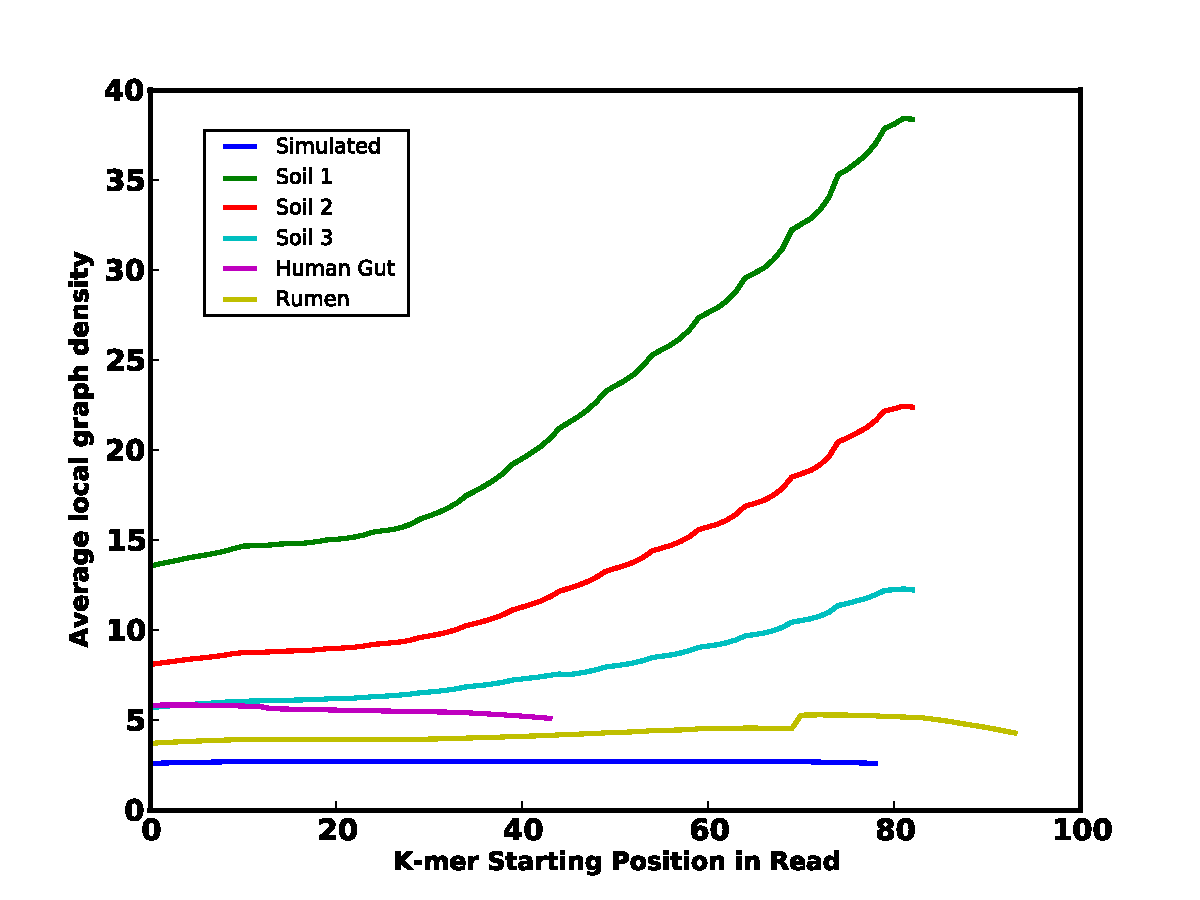
\includegraphics[width=5in]{./Figures/density_pos.pdf}}
\caption{The extent to which average local graph density varies by read position is shown for the lump of various datasets.  Unlike the graph density of the simulated metagenome lump, average graph density of sequences in metagenomic lumps varied significantly by position along the read.}
\end{figure}

\begin{figure}
\center{\includegraphics[width=5in]{./Figures/position_read_stoptags.pdf}}
\caption{The extent to which highly-connecting k-mers (solid lines) and the subset of highly abundant (> 50) k-mers (dashed lines) are present at specific positions within sequencing reads for various metagenomes.}
\end{figure}


\begin{figure}
\center{\includegraphics[width=5in]{./Figures/contig_pos_stoptags.pdf}}
\caption{When incorporated into an assembly, highly-connecting sequences (k-mers) were disproportionately present at the ends of contigs.}
\end{figure}


\end{document}







